\section{Local search heuristics for TSP}

\subsection{Disposition}

\textbf{TODO: } Den her var jeg personligt selv op i. Vær opmærksom på de nok spørger om Lin Kernighan, så få styr på den. Disse noter indeholder ikke noget af betydning om den. Desuden var der kritik af der gik for lang tid før jeg snakkede om det relevante i emnet, så spring meget hurtigt over de første 2 punkter eller helt undlad dem. 

\begin{enumerate}
 \item \textbf{Def. P, NP, NP-hard \& NPC}
    \subitem  Tegn og MEGET hurtig def.
 \item \textbf{Løsning af NPC problemer}
    \subitem Direkte løsning (exp time)
    \subitem Special cases
    \subitem Approximation Algoritmer \& Heuristics
  \item \textbf{Local search heuristics}
    \subitem Hvordan finder vi den initielle kandidatløsning?
    \subitem Hvordan skal neighborhood designet være?
    \subitem Hvilken nabo skal vælges i en given iteration?
    \subitem Hvornår skal vi terminere?
 \item \textbf{Def. TSP}
 \item \textbf{Teoretiske begrænsninger}
    \subitem Generel TSP ($A(I)/OPT(I) \leq 2^{p(n)}$)
    \subitem Metric TSP ($A(I)/OPT(I) \leq 1+\varepsilon$)
    \subitem Bedst kendte performancegaranti ($A(I)/OPT(I) \leq 1.5$)
 \item \textbf{Held Karp lower bound}
    \subitem Emperisk sammenligningsgrundlag (min. $2/3$ af optimal tur ved metric TSP)
 \item \textbf{Tour Construction Heuristics}
    \subitem Christofides
    \subitem Greedy heuristics
    \subitem Nearest neighbor heuristic
    \subitem Clarke-Wright
    \subitem Random
 \item \textbf{Lokale Optimeringsalgoritmer}
    \subitem 2-opt
    \subitem 3-opt
    \subitem Hastighedsforbedringer (neighbor lists, pruning lists)
\end{enumerate}

\subsection{Emne detaljer}

Følgende afsnit indeholder detaljer om hvert punkt i dispositionen ovenfor (og muligvis flere ting også).

\subsubsection{Def. P, NP, NP-hard \& NPC}

Lad os starte med lige at kigge på de kompleksitetsklasser vi har arbejdet med her i kurset.
\begin{center}
 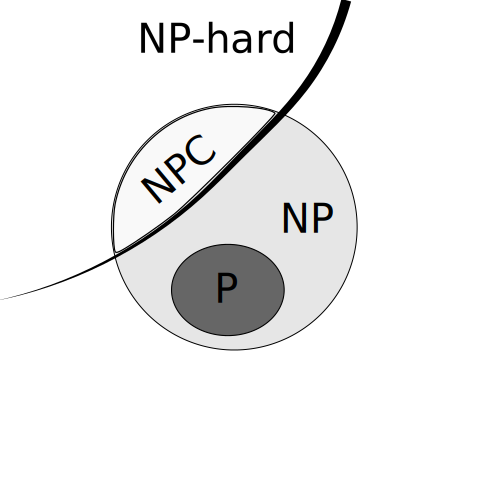
\includegraphics[bb=0 0 400 400,scale=0.3]{img/PNPNPC.png}
 % PNPNPC.png: 1667x1667 pixel, 300dpi, 14.11x14.11 cm, bb=0 0 400 400
\end{center}


\paragraph{P}
~\\
~\\
Kompleksitetsklassen $P$ er formelt defineret således:
\begin{align*}
 P = \left\lbrace L \subseteq \left\lbrace 0,1 \right\rbrace^* | \exists \text{ TM } M_L \text{ der afgører L i polynomiel tid } \right\rbrace
\end{align*}
Altså klassen af beslutningsproblemer der kan blive bestemt af en deterministisk Turing Maskine hvor antallet af ``steps'' maskinen udfører for et givent $x$ maksimalt er $\rho(x)$ for et givent polynomiel $\rho$.\\
 
Intuivit ser vi kompleksitetsklassen $P$ som en klasse for problemer for hvilket vi kender en effektiv løsning. Altså ethvert problem med worst-case kørselstid på formen $O(n^k)$ for et givent $k$.

At worst-case kørseltid på et problem er polynomiel betyder dog ikke reelt at det er et nemt problem (modsat hvad Cobham's Thesis påstår). I hele den analyse ignorerer vi fuldkommen konstanter, samt forventet kørselstid som I mange tilfælde kan få ``sværere'' problemer til at køre bedre end ``nemme'' problemer i $P$.


\paragraph{NP}
~\\
~\\
Kompleksitetsklassen $NP$ er lidt mere kluntet formelt defineret, så vi starter lige med intuitionen først.

Intuitivt kan $NP$ ses som klassen af beslutningsproblemer for hvilket ``yes'' instanserne kan verificeres i polynomiel tid på en deterministisk Turing Maskine. Altså er det komplekse problemer med eksponentiel løbetid, men hvor løsningen til et sådant problem nemt kan verificeres til at være korrekt.\\
~\\
Kompleksitetsklassen $NP$ er formelt defineret således:
\begin{align*}
 NP = \left\lbrace L \subseteq \left\lbrace 0,1 \right\rbrace^* | \exists \rho \in Z[x], L' \in P, \forall x \in \left\lbrace 0,1 \right\rbrace^* : ( x \in L \Leftrightarrow \exists y \in \left\lbrace 0,1 \right\rbrace^* : |y| \leq \rho(|x|) \wedge \left\langle x,y \right\rangle \in L') \right\rbrace
\end{align*}
Definitionen skal forståes således: Vi har et sprog $L' \in P$, samt et polynomiel $\rho$. Vi tænker så nu på et sæt af binære strenge af længde maksimalt $\rho(|x|)$, hvor disse representerer mulige løsninger til probleminstansen $x$. Med denne fortolkning bliver $\left\langle x,y \right\rangle \in L'$ så måden hvorpå vi tester om en given løsning $y$ virkelig er en korrekt løsning. 

Denne form for søgningsproblem kaldes ofte for et simpelt søgningsproblem, da den kan verificeres i polynomiel tid, men ikke løses deri (antaget $P \neq NP$).\\

For at løse et givent NP problem kunne vi så løbe igennem alle mulige løsninger for $y$, som sammenlagt ville være $2^{\rho(|x|)+1}-1$, og for hver af dem tjekke $\left\langle x,y \right\rangle \in L'$. Det ønsker vi dog ikke, da det ville tage eksponentiel tid. I stedet forsøger man ofte at finde snedige måder at lave speed-ups og/eller lave approximationsalgoritmer af forskellige art.

Og i visse tilfælde er man også heldig at finde en algoritme i $P$ for et $NP$ problem, hvorved man har vist at problemet i virkeligheden ligger i $P$ som jo er et subset af $NP$.

\paragraph{NP-hard}
~\\
~\\
Et sprog defineres som NP-hard såfremt der gælder:

\begin{align*}
 \forall L' \in NP: L' \leq L
\end{align*}

Altså gælder der, at ethvert sprog $L'$ i NP kan reduceres til $L$. Intuitionen er her, at algoritmen til at løse NP-hard problemet er så stærk (eller generel) at den kan bruges til at løse ethvert andet problem i NP. Man siger desuden, at et NP-hard problem således er mindre sandsynlig end noget andet sprog i NP, til at være i P.\\

Navnet kan dog være lidt forvirrende, da et NP-hard problem faktisk ikke behøver være i NP og hvis de er, så kaldes de faktisk ikke engang bare NP-hard længere.

\paragraph{NPC}
~\\
~\\
NP-Complete (NPC) er den særlige klasse af problemer der både er NP-hard og befinder sig i NP. Formelt defineret således: 

\begin{align*}
 NPC = \left\lbrace L \in \left\lbrace 0,1 \right\rbrace^* | L \in NP \wedge (\forall L' \in NP: L' \leq L) \right\rbrace
\end{align*}

NPC problemer er særligt interessante, da vi kan bruge dem til at bevise et givent problem er NP-Complete, således vi ikke spilder tid på forsøg med at finde en algoritme i $P$ for problemet (antaget $P\neq NP$). Dette gør vi vha. noget vi kalder reduktioner.


\subsubsection{Løsning af NPC problemer}

Men hvad så hvis vi har et givent NPC problem og vi egentlig gerne vil løse det og ikke bare bruge det til at vise andre problemer er i NPC? Så har vi grundlæggende 3 muligheder vi kan benytte os af:

\begin{description}
 \item[Direkte løsning:] Hvis vi har et meget lille input, så kan det måske være fint at bruge algoritmen direkte og så leve med den eksponentielle kørselstid. En sådan algoritme vil dog ofte i praksis være fuldkommen umulig at udregne direkte i ens levetid, selv for rimelig små input. Der er dog også tilfælde hvor algoritmer med worst-case eksponentiel kørselstid har langt bedre kørselstid i praksis, hvorfor direkte exact løsning er fint.
 \item[Isoler special cases:] Flere NPC problemer har special cases der kan løses i polynomiel tid. Man kunne bruge det problem i stede såfremt den specifikke special case løser ens problem.
 \item[Approximation \& Heuristics:] Hvis de to ovenstående løsninger ikke er mulige, så kan man i stedet forsøge at finde ``nær-optimale'' løsninger i polynomiel tid vha. approximationsalgoritmer eller heuristikker.
\end{description}

Vi vil i dette emne fokusere på de såkaldte local search heuristikker til løsning af TSP problemet.


\subsubsection{Local search heuristics}

Local search er et kendt algoritmemønster til optimering, som bruges i en lang række algoritmer indenfor adskillige felter. Mønsteret kan generelt anvendes på problemer hvor formålet kan formuleres som at maksimere et givent kriterie iblandt et antal kandidatløsninger i et såkaldt ``search space''.

 Eksempler på algoritmer der bruger local search er:
\begin{itemize}
 \item Ford-Fulkerson (Max Flow)
 \item Klein's Algoritme (Min Cost Flow)
 \item Simplex Algoritmen (Linear Programming)
 \item K-Means Clustering
 \item ... m.fl.
\end{itemize}
Local search algoritmen kan opskrives således:
\begin{center}
 \includegraphics[bb=0 0 218 132]{img/localSearch.png}
 % localSearch.png: 291x176 pixel, 96dpi, 7.70x4.66 cm, bb=0 0 218 132
\end{center}
Så local search starter altså på en eller anden kandidatløsning og bevæger sig herefter fra løsning til løsning i mængden af kandidatløsninger. Dette bliver den ved med indtil den løsning den opfatter som optimal eller en givent timeout er nået.\\
~\\
Vi skal så nu kigge på en række local search heuristikker til TSP, hvor svarene til følgende spørgsmål varierer for de givne algoritmer:
\begin{enumerate}
 \item Hvordan finder vi den initielle kandidatløsning?
 \item Hvordan skal neighborhood designet være?
 \item Hvilken nabo skal vælges i en given iteration?
 \item Hvornår skal vi terminere?
\end{enumerate}

Inden vi går videre med det, så bør vi dog lige først definere TSP problemet vi har at gøre med og kigge på de teoretiske begrænsninger vi ved der eksisterer for heuristikkers performance for TSP.

\subsubsection{Def. TSP}

Problemet hedder Traveling Salesman Problem, eller forkertet TSP, og går ud på følgende:\\
~\\
\textbf{TSP:} Givet en $n \times n$ positiv distancematrix $d_{ij}$, find en permutation $\pi$ på $\left\lbrace 0,1,2,\hdots,n-1 \right\rbrace$ der minimerer:
\begin{align*}
 \sum_{i=0}^{n-1} d_{\pi(i), \pi(i+1 \text{ mod } n)}
\end{align*}
OBS: mod $n$ delen ovenfor gør blot, at vi definerer en cycle, i det at for $n=4$ der får vi $n-1=3$ så $(3+1 \text{ mod } 4)=0$.

\paragraph{Euclidean TSP}
~\\
~\\
Der er desuden en række special cases af TSP, som eksempelvis Euclid TSP hvor $d_{ij}$ er deciderede distancer på et givent kort. Vær opmærksom på input til dette problem ikke er distancerne, men derimod blot punkterne på det givne kort. Distancerne behandles derved implicit.\\

\paragraph{Metric TSP}
~\\
~\\
Endnu en special case har vi så i metric TSP hvor $d_{ij}$ tilfredsstiller den såkaldte trekantsulighed. Trekantsuligheden sikrer at, man populært sagt ikke kan lave genveje, således at en direkte vej fra by $i$ til by $j$ aldrig er længere end en omvej via. en tredje by $k$. Eller skrevet lidt mere formelt op:
\begin{align*}
 d_{\pi(i),\pi(j)} \leq d_{\pi(i),\pi(k)} + d_{\pi(k),\pi(j)}
\end{align*}
~\\
Medmindre andet nævnes i gennemgangen herefter, så vil vi som udgangspunkt antage at vi har instanser af metric TSP (således trekantsuligheden gælder), og laver desuden den yderligere begrænsning kun at kigge på symmetriske varianter af TSP, således $d_{\pi(i),\pi(j)} = d_{\pi(j),\pi(i)}$.


\subsubsection{Teoretiske begrænsninger}

Som det også bliver beskrevet i det case-study vi har haft i løbet af kurset (Johnson and McGeoch), så er der visse teoretiske begrænsninger for kvaliteten af vores heuristikker.

For en given heuristik $A$ og en TSP instans $I$, så lad $A(I)$ være længden af turen produceret af $A$ og lad $OPT(I)$ være længden af den optimale tur. Hvis vi ikke havde begrænset hvilke typer instanser af TSP vi kiggede på, så ville vi have haft en bedste performancegaranti på $A(I)/OPT(I) \leq 2^{p(n)}$ for ethvert givet polynomie $p$ og all instanser $I$. Men heldigvis fokuserer vi på metric TSP instanser, således det i stedet er følgende begrænsning:\\
~\\
\textbf{Theorem B:} Antaget $P \neq NP$, så eksisterer der et $\varepsilon > 0$ således at ingen polynomieltids TSP heuristik kan garantere bedre performance end $A(I)/OPT(I) \leq 1+\varepsilon$ for alle instanser $I$ der tilfredsstiller trekantsuligheden.\\
~\\
Selv denne lower bound på vores performance forsvinder dog, hvis vi kun kigger på euclid instanser af TSP, da Arora(1996) så har bevist der eksisterer polynomieltids approximations schemes (PTAS) for TSP. Som skrives i theoremet således:\\
~\\
\textbf{Theorem C:} Der er en algoritme $A$ således, at givet en euclidisk TSP instans og en konstant $\varepsilon > 0$, så har $A$ kørselstid $n^{O(\frac{1}{\varepsilon})}$ og garanterer performance $A(I)/OPT(I) < 1+\varepsilon$.\\
~\\
Desværre er resultatet dog kun teoretisk interessant, da konstanterne involveret er for store og fordi den kræver lige så meget plads som tid (pladsforbruget er altså: $n^{O(\frac{1}{\varepsilon})}$). 

Så vores teoretiske nedre grænse vil være den der defineres i Theorem B, nemlig $A(I)/OPT(I) \leq 1+\varepsilon$. Hvor den bedst kendte algoritme pt. (ifølge case storien) har performancegaranti $A(I)/OPT(I) \leq 1.5$.

\subsubsection{Held-Karp lower bound}

Når vi skal sammenligne forskellige empiriske resultater for algoritmeperformance, så har vi sjællendt mulighed for at beregne på baggrund af den reele optimale turlængde, da vi simpelthen ikke kender den for tilstrækkeligt store instanser. Så i stedet gør man det (som også case studien gør) at man sammenligner med et lower bound på den optimale længde kaldet Held-Karp lower boundet.

Held-Karp lower boundet kan beregnes væsentligt nemmere, da det er løsningen til en standard lineær programmerings-relaxation af TSP. Dog kan man få problemer med at udregne den for tilstrækkeligt store instanser da antallet af constraints i programmet er eksponentielt i $n$. Så i stedet vil man normalt lave nogle snedige tricks med at dele LP programmet op i en række begrænsede LP problemer hvor hver kun indeholder et subset af de givne constraints, efterfulgt af yderligere snedige tricks med at identificere constraintbrud og proppe dem med i næste LP i kæden osv. Generelt så kompliceret at case storien heller ikke gad andet end nævne det og vi ved blot, at det er blevet brugt til at udregne Held-Karp for instanser på op til $33810$ byer. For instanser større end $33810$ lever vi med en approximation på Held-Karp.\\

Held-Karp lower boundet er således garanteret til at være minimum $2/3$ af den optimale værdi antaget metric TSP, og i praksis er den ofte langt bedre (typisk inden for $0.01\%$).

\subsubsection{Tour Construction Heuristics}

Nu hvor alt forarbejdet er lavet, så kan vi så komme i gang med at kigge på opbygningen af en reel heuristik til TSP. Som vi identificerede da vi kiggede på local search spørgsmålene, så skal vi besvare følgende spørgsmål:
\begin{center}
 \textit{Hvordan finder vi den initielle kandidatløsning?}
\end{center}
Og svaret er for TSP: Tour Construction Heuristics!

Der er mange forskellige måder at lave disse tour construction heuristics på, men vi blev i case studiet introduceret til 4 direkte og 1 implicit. Disse var:

\paragraph{Nearest Neighbor}
~\\
~\\
I NN, eller Nearest Neighbor, vælger man den initielle by i ens tour tilfældigt hvorefter man fra en given by $i$ vælger næste by $k$ til at være den der minimerer $d_{\pi(i),\pi(k)}$. Altså sagt på en anden måde: Altid vælg den ubesøgte by der er tættest på fra der hvor du er nu. Hermed får man en tour der går igennem alle byer og ender hvor man startede.

Kørselstiden på NN er $\Theta(n^2)$. Den bedste performancegaranti vi får på NN er $NN(I)/OPT(I) \leq 0.5(\lfloor \log_2 N \rfloor + 1)$. Ingen bedre garanti er mulig, da der findes instanser hvor forholdet stiger med $\Theta(\log n)$.

Mht. emperiske resultater fra case studiet, så viser det sig, at NN klarer sig markant dårligere end de 3 andre algoritmer ved tour construction på tilfældige euclidiske instanser hvad angår turkvalitet. NN var imellem $23.3\%$ og $26.2\%$ over Held-Karp lower bound, afhængig af antal byer $n$ (NN blev bedre for større $n$).

\paragraph{Greedy}
~\\
~\\
I Greedy er der lidt en anden tilgang til problemet, i det at man antager byer allerede er organiseret som en graf hvor byerne er knuder og længden af kanten imellem by $i$ og $j$ er $d_{\pi(i),\pi(j)}$ for alle byer $i$ og $j$. En tour er således nu blot en Hamilton Cycle igennem grafen hvor alle knuder (byer) har degree 2 (i.e. de er forbundet til 2 kanter).

Man bygger så denne cycle op ved at tilføje kanter til touren en efter en, startende fra den korteste kant og derefter tilføje den næstkorteste frie kant, tredjekorteste frie kant osv. Hvor en fri kant er en kant der endnu ikke er i touren og som, ved at blive tilføjet, ikke skaber en knude med degree 3 eller en cycle på på længde mindre end $n$.

Kørselstiden på Greedy kan implementeres til at være $\Theta(n^2 \log n)$ og er derved en anelse langsommere end NN, men har så en worst-case turkvalitet der muligvis er lidt bedre. Mht. bedste performancegaranti har den $greedy(I)/OPT(I) \leq 0.5(\lceil \log_2 n \rceil + 1)$ , men dens worst-case instanser hvad angår turkvalitet får kun forholdet til at stige $\frac{(\log n)}{(3 \log \log n)}$.

Mht. emperiske resultater fra case studiet, så klarer Greedy sig lidt bedre end NN i praksis hvad angår turkvalitet ved tour construction på tilfældige euclidiske instanser. NN var som sagt imellem $23.4\%$ og $26.2\%$ over Held-Karp lower bound, hvor Greedy var imellem $14.2\%$ og $19.5\%$, igen hvor kvaliteten forøges med størrelsen af $n$.

\paragraph{Clarke-Wright}
~\\
~\\

Clarke-Wright, forkortet CW, er lidt mere speciel. Vi starter med en såkaldt pseudotour hvor en arbitrær by vælges til at være ``hub'' og sælgeren kommer så tilbage til denne hub efter hvert besøg til en anden by. Altså starter vi med en multigraf hvor alle andre ikke-hub byer er forbundet til hubben med 2 kanter. 

For hvert par af ikke-hub byer $i$ og $j$, der definerer vi så en ``savings'' som er den distance der ville blive sparet såfremt sælgeren gik direkte fra by $i$ til by $j$ ved at gå uden om hubben. Herefter bliver algoritmen ligesom Greedy i den forstand, at den går igennem ikke-hub byerne i par af faldende grad af savings og går uden om hubben sålænge det ikke skaber en cycle af ikke-hub byer og ikke får en ikke-hub by til at være ved siden af mere end to andre ikke-hub byer. 
Konstruktionen bliver ved indtil vi kun har to ikke-hub byer stadig forbundet til hubben, hvorefter vi har en komplet tour.

Ligesom med Greedy så er kørselstiden $\Theta(n^2 \log n)$. Mht. bedste performancegaranti er den dog en helt faktor 2 bedre end Greedy, så $CW(I)/OPT(I) \leq \lceil \log_2 n \rceil + 1$, men de værste kendte eksempler får stadig samme forhold $\frac{(\log n)}{(3 \log \log n)}$ ligesom med Greedy.

Mht. emperiske resultater fra case studiet, så klarer Clarke-Wright sig markant bedre, hvad angår turkvalitet, end både Greedy og NN på tilfældige euclidiske instanser. Clarke-Wright var imellem $9.2\%$ og $12.2\%$ over Held-Karp lower bound, hvilket er markant bedre end eksempelvis Greedys $14.2\%$ og $19.5\%$. Modsat NN og Greedy, så bliver Clarke-Wright dog dårligere med større $n$, således turkvaliteten er bedst for små instanser.

\paragraph{Christofides}
~\\
~\\

Alle de tidligere 3 algoritmer have worst-case approximations ratios der steg med $n$, selv når trekantsuligheden holdte. Vi er stadig langt fra den teoretiske grænse som blev sat af Theorem B, og i virkeligheden er der også mange andre algoritmer der giver langt bedre resultater.

En af disse er Christofides, som pt. er den bedste kendte tour construction heuristic hvad angår worst case approximations ratio, med et worst case forhold på bare $\frac{3}{2}$ antaget trekantuligheden. Algoritmen virker således:
\begin{enumerate}
 \item Konstruer et minimum spanning tree $T$ for sættet af byer (OBS: læg mærke til, intet sådant træ kan være længere end $OPT(I)$, siden det at slette en kant fra en optimal tour giver et spanning tree)
 \item Herefter skaber vi en minimum længde perfect matching $M$ af knuderne med ulige degree i $T$. Denne matching vil ikke være længere end $OPT(I)/2$.
 \item Herefter kombinerer vi $M$ og $T$, hvor vi får en forbundet multigraf hvor hver knude har lige degree.
 \item Denne graf indeholder nu en Euler tour, i.e. en cycle som går igennem hver kant præcis en gang, og denne finder vi. (\textbf{TODO: } Hvordan?)
 \item En TSP tour kan nu konstrueres ved at traversere denne cycle og tage ``genveje'' for at undgå dobbeltbesøgte knuder. En genvej ersatter en rute imellem to byer med en direkte kant imellem de to. Denne nye kant skal dog overholde trekantuligheden, således den ikke kan være længere end den den erstatter. 
\end{enumerate}

Denne algoritme giver så den bedste approximations ratio for alle kendte algoritmer, men den giver også gode resultater i praksis. Dog er den dyr i kørselstid, i det at dens matching skridt i sig selv tager $\Theta(n^3)$. Der er dog teoretiske måder at forbedre denne kørselstid lidt på, så den bliver $\Theta(n^{2.5})$ (de er dog aldrig blevet implementeret ifølge case studiet).

Mht. emperiske resultater fra case studier, så klarer Christofides sig bedre end alle andre algoritmer, med tourkvalitet kun $9.5\%$ til $9.9\%$ over Held-Karp lower bound, og ligesom med Clarke-Wright, så bliver kvaliteten lidt dårligere med større $n$, men ved Christofides er den mere stabil (Kun $0.4$ procentpoint fra bedste til dårligste). Der betales dog også godt for denne ekstra kvalitet, da dens emperiske resultater for kørselstid giver den en markant længere kørselstid end alle andre algoritmer allerede fra $n=10^{3}$


\paragraph{Random}
~\\
~\\

Og så sidst men ikke mindst, den case studiet kun fremviste implicit ved at bruge den som sammenligningsgrundlag - fuldkommen random tour construction.

Som man nok kunne forestille sig, så virker det dog ikke fantastisk i forhold til de andre tour construction algoritmer - i hvert fald ikke hvis det er der man stopper i ens opbygning. Average excess over Held-Karp for Random var $2150\%$ ved tilfældige euclidiske instanser og $24500\%$ ved tilfældige distancematricer. 

Random tour construction virker dog forbavsende godt alligevel hvis brugt i kombination med 2-opt eller 3-opt som jeg beskriver senere.


\subsubsection{Lokale Optimeringsalgoritmer}

Nu har vi så en initiel kandidatløsning konstrueret ud fra Nearest Neighbor, Greedy, Clarke-Wright, Christofides eller måske endda bare Random genereret. Nu er det så vi skal kigge på et par lokale optimeringsalgoritmer der givet en kandidatløsning laver iterationer af små ændringer i touren der forkorter dens længde, indtil en tour nås hvor ingen ændring giver en forbedring - en lokalt optimal tour. 

Dette kan også, lidt mere i local search terminologien, ses som en ``neighborhood search'' proces hvor hver tour har et associeret nabolag af tilstødende tours, i.e. dem der kan nås i et enkelt ``move'' eller operation. Man bliver så kontinuert ved med at flytte sig til en bedre nabo indtil ingen bedre nabo eksisterer.\\
~\\
De simpleste af disse algoritmer er 2-Opt og 3-Opt.\\

\paragraph{2-Opt}
~\\
~\\
2-Opt går ud på at slette 2 kanter, for derved at splitte touren i to, og så sætte dem sammen igen på en ny måde. Den sætter dem dog kun sammen igen, såfremt denne handling forbedrer tourens længde. Således kunne man have følgende situation:
\begin{center}
 \includegraphics[bb=0 0 313 204,scale=0.5]{img/2opt1.png}
 % 2opt1.png: 417x272 pixel, 96dpi, 11.03x7.20 cm, bb=0 0 313 204
 \includegraphics[bb=0 0 313 204,scale=0.5]{img/2opt2.png}
 % 2opt1.png: 417x272 pixel, 96dpi, 11.03x7.20 cm, bb=0 0 313 204
\end{center}
Vi har altså planer om at slette de markerede kanter for at lægge dem på en anden måde. Vi tjekker derfor:
\begin{enumerate}
 \item Hvis $d_{\pi(t_1), \pi(t_2)} \leq d_{\pi(t_2), \pi(t_3)}$ og $d_{\pi(t_3), \pi(t_4)} \leq d_{\pi(t_4), \pi(t_1)}$ så forbedrer skiftet intet og udføres derfor ik.
 \item Hvis $d_{\pi(t_1), \pi(t_2)} > d_{\pi(t_2), \pi(t_3)}$ eller $d_{\pi(t_3), \pi(t_4)} > d_{\pi(t_4), \pi(t_1)}$ så vil vi derimod kunne forbedre touren, hvorfor skiftet laves så vi kommer til situationen nedenfor.
\end{enumerate}
\begin{center}
 \includegraphics[bb=0 0 313 204,scale=0.5]{img/2opt3.png}
 % 2opt1.png: 417x272 pixel, 96dpi, 11.03x7.20 cm, bb=0 0 313 204
\end{center}

Hvad angår kørselstid, så er den ikke fantastisk da størrelsen af nabolaget for en $k$-Opt algoritme er $O(n^k)$. Så i praksis udføres der normalvis snedige og komplekse implementationer der sikrer algoritmen kører så hurtigt som muligt. Nogle få af de tiltag kommer jeg ind på om lidt.


\paragraph{3-Opt}
~\\
~\\
3-Opt fungerer ligesom 2-Opt, bortset fra den skifter 3 kanter af gangen i stedet for 2. Hvad angår kørselstid så følger den samme $k$-Opt algoritme kørselstid, så $O(n^3)$ for 3-Opt.


\paragraph{Emperiske studier}
~\\
~\\
Hvad angår de emperiske resultater af 2-Opt/3-Opt brug i case studiet, så ser vi at begge havde meget positiv effekt på den endelige tour-kvalitet. Faktisk viste Random tour construction sig lige pludselig også okay, i det at tourkvaliteten for denne faktisk var bedre end Clarke-Wright både ved 2-Opt og 3-Opt. 

Faktisk kan vi se et resultat, som case studiet også underbygger er generelt sandt, nemlig at Greedy tour construction giver de bedste endelige resultater for 2-Opt og 3-Opt for alle kendte tour construction heuristics. Faktisk kan det ses, at lokal optimering kun giver kraftige forbedringer såfremt udgangspunktet er tilstrækkeligt befængt med defekter. Derved giver selv den optimale Christofides faktisk dårligere resultater end Greedy, når 2-Opt og 3-Opt køres på den efterfølgende (ifølge case studiet - det fremgår ikke af graferne).


\paragraph{Hastighedsforbedringer}
~\\
~\\
2-Opt og 3-Opt er som sagt langsomme metoder, da størrelsen af nabolaget vokser med $O(n^k)$ for alle $k$-Opt algoritmer. Derfor kan det at vælge et godt 2-Opt move pludselig blive en meget kostelig affære. Der er dog måder at forbedre dette:

\begin{description}
 \item[Neighborhood lists:] For hver by gemmes der en statisk liste af alle byer sorteret med stigende distance. Dette muliggører forventet lineærtids søgning efter et 2-Opt ``move''.
 \item[List pruning:] Selv neighborhoodlister kan blive ret store og det er sjællendt det er relevant at kigge på byer ved position $> 20$ i listen. Så cut listen ned til de 20 tætteste byer. Kun hvis vi efter at have gået igennem alle disse 20 byer ikke finder et forbedrende ``move'' går vi ud og søger i hele ``search space''. 
\end{description}

Der er også en række andre muligheder, så som ``Don't look bits'', men dem vil vi ikke komme ind på her.

\subsubsection{Nye optimeringstilgange}

Lad os så antage vi har fået tour construction og local search til at køre fantastisk, og det hele er bare fint og sågar praktisk og alt muligt. Så har vi dog et problem: Hvad hvis et givent ``search space'' indeholder flere lokale optimums der er kraftigt dårligere end den globalt optimale? Hvordan undgår vi, at vores local search sætter sig fast ved en sådan dårligere løsning?

Måden hvorpå vi gør det, er at modificere vores local search algoritmer, således de har mekanismer til at flygte fra lokale optimums. En simpel måde at implementere dette på ville blot være ved at bruge normalt 2-Opt og 3-Opt, men så bruge en tour construction heuristic med et niveau af tilfældighed i, således vores udgangspunkt var forskellige for hver gang man kørte algoritmen. Således kunne vi bare køre hele algoritmen med k-Opt moves og det hele igen og igen, indtil vi var tilfreds med den løsning vi fik. 

En anden mulighed er at bruge varianter på local search der forsøger at finde globalt optimale løsninger. Vi har overordnet 4 forskellige algoritmer til dette formål:

\begin{itemize}
 \item Taboo search
 \item Lin-Kernighan
 \item Simulated annealing
 \item Evolutionary algorithms
\end{itemize}

Vi vil kun beskrive algoritmer meget overordnet og kan initielt sige, at Johnson \& McGeoch konkluderede at følgende var de bedste kendte heuristikker for TSP (alt afhængig af hvor meget tid du vil bruge på at beregne):
\begin{itemize}
 \item Lille CPU-tid: Lin-Kernighan
 \item Medium CPU-tid: Iterated Lin-Kernighan
 \item Meget stor CPU-tid: En evolutionsalgoritme
\end{itemize}


\paragraph{Taboo search}
~\\
~\\
Taboo search er en variation på local search hvor vi givet et lokalt optimum bliver ved med at søge, således vi egentlig laver et move der ikke forbedrer løsningen, men derimod forringer den. Hvis vi så ikke gør mere nu, så vil algoritmen typisk gå ind i en cycle af længde 2, da den vil hoppe ud og ind af et lokalt optimum. Derfor klacificerer vi træk vi har lavet for ``taboo'' således de ikke må udføres igen i et givent tidsrum herefter. Dette gør vi typisk vha. lister af tidligere sette løsninger, hvilket dog ikke er vildt praktisk, da disse lister ender med at blive ret store.

Når alt kommer til alt så er det heller ikke vildt nyttigt for TSP, da ingen ``ren'' variant af taboo search virker særlig godt for TSP i praksis (i hvert fald ikke en man har fundet endnu). For instanser af størrelse $1000$ fandt (Johnson \& McGeoch) at Taboo search havde omtrent samme kørselstid som 3-Opt, men uden nogen betydningsfulde forbedringer.


\paragraph{Lin-Kernighan}
~\\
~\\
Lin-Kernighan er en anden variant, der er mere eller mindre kendt for at være kongen af TSP optimization algoritmer. Den er pænt kompleks og tager lang tid at gennemgå, så det vil jeg ikke umiddelbart gøre. Ikke udover det plan, at sige, at det er en generalisering af 2-Opt og 3-Opt, og så har den desuden en række restriktioner indbygget - bl.a. et taboo komponent.

Ifølge (Johnson \& McGeoch) klarer den sig bedre end nogen anden algoritme hvad angår endelig turkvalitet og den kører sågar relativt hurtigt, ved at den kan håndterer instanser med op til 1 million byer i løbet af 55 minutter.\\

(OBS: Der er en variant på Lin-Kernighan kaldet Iterated Lin-Kernighan, hvor man laver normal Lin-Kernighan + tilfælde 4-opt moves.) 


\paragraph{Simulated Annealing}
~\\
~\\
Simulated Annealing er speciel i det at den afhænger meget af sandsynlighed. Den vil, ligesom andre algoritmer her, til tider tage et skridt der ikke forbedre touren for at kunne komme ud af lokale optimums, men den vil også i visse tilfælde gøre det selvom den ikke er i et lokalt optimum. Overordnet går den ud på at vælge en given løsning fra nabolaget med en sandlighed udregnet på baggrund af differencen i tourkvalitet opnået samt en global ``temperatur'' $T$ som falder i løbet af udførslen. $T$ vælges så initielt til en given værdi alt afhængig af hvad man vil opnå:
\begin{description}
 \item[T er stor:] Konvergerer mod en grænsefordeling hurtigt, men grænsefordelingen favoriserer ikke gode løsninger særlig meget. Hvis $T=\infty$ er søgningen random)
 \item[T er tæt på 0:] Grænsefordelingen favoriserer gode løsninger, men konvergeringen er langsom.
 \item[T er 0:] Helt normal local search
\end{description}


\paragraph{Evolutionary Algorithms}
~\\
~\\
En sidste type algoritme til at løse dårlige lokale optimum problemet er Evolutions/Genetiske algoritmer. Overordnet går det ud på følgende trin:
\begin{enumerate}
 \item Håndter en befolkning af løsninger.
 \item Muter løsninger for at opnå nye
 \item Rekombiner løsninger, for at opnå nye
 \item Dræb løsninger tilfældigt, med stærkere/bedre (mere ``fit'') løsninger havende lavere sandsynlighed for at dø.
\end{enumerate}
Ideen er, som det også ses ret tydeligt, at modellere biologiske systemer. 

Evolutionsalgoritmer er dog også dybt komplekse, så vi vil ikke gå i flere detaljer med det her.







